%%=============================================================================
%% Inleiding
%%=============================================================================

\chapter{\IfLanguageName{dutch}{Inleiding}{Introduction}}%
\label{ch:inleiding}
Amerikaanse investeringsmaatschappijen met een jaaromzet van ten minste USD 100.000.000, zoals Soros Fund Management, Appaloosa Management en Berkshire Hathaway, zijn periodiek verplicht hun financiële posities te rapporteren aan de Securities and Exchange Commission (SEC). Dit doen ze onder andere via de zogenaamde 13F-meldingen. Deze meldingen worden opgeslagen in de EDGAR-database\footnote{\href{https://www.sec.gov/edgar/search/\#/dateRange=custom\&category=custom\&startdt=2001-01-01\&enddt=2012-12-31\&forms=13F-HR}{SEC EDGAR zoeken voor 13F-HR meldingen (2001-2012)}}\footnote{\href{https://www.sec.gov/edgar/search/}{SEC EDGAR zoeken thuispagina}}
 en zijn openbaar toegankelijk. Enkel 13F meldingen van na 1 januari 2001 zijn beschikbaar in de EDGAR databank.


Regelgevende filings van institutionele beleggers, zoals pensioenfondsen en vermogensbeheerders, bieden belangrijke inzichten in marktpatronen en beleggingsstrategieën. Ze vormen vaak de basis voor het genereren van aan- en verkoopsignalen op beurzen zoals de NYSE en Nasdaq. De informatie die in deze registraties wordt weergegeven, is van cruciaal belang voor financieel onderzoek en beleggingsanalyses. 

13F-meldingen van voor 2013 brengen echter aanzienlijke uitdagingen met zich mee vanwege hun variabele vormen en structuren, wat de verwerking en analyse ervan bemoeilijkt. Tot die tijd werden de meldingen ingediend als "flat files", oftewel .txt-bestanden, zonder strikte regels over de locatie van specifieke informatie. Dit maakt het systematisch extraheren van nuttige gegevens lastig.

De opkomst van geavanceerde AI-technologie biedt mogelijkheden om deze problemen aan te pakken. Natural Language Processing (NLP) en Machine Learning (ML) bieden geavanceerde methoden om gegevens uit ongestructureerde tekst te extraheren en te organiseren. Deze technologieën kunnen het proces van het standaardiseren en integreren van vroegere 13F-meldingen in een goed georganiseerde relationele databank automatiseren, wat de toegang en het gebruik van deze gegevens aanzienlijk zou verbeteren.

Sinds 2013 verplicht de SEC bedrijven om hun rapporten in .xml-formaat in te dienen, wat de structuur van de gegevens aanzienlijk heeft verbeterd. Toch blijven de gegevens van voor 2013 belangrijk, omdat ze kunnen dienen als testdata voor het ontwikkelen van beleggingsstrategieën.

Dit proefschrift richt zich op het ontwikkelen van een proof of concept toepassing die NLP en ML-technieken gebruikt om 13F-meldingen van voor 2013 te standaardiseren en te integreren in een relationele databank. Het doel is om het proces van gegevensextractie te stroomlijnen door de meldingen automatisch om te zetten in een gestandaardiseerd formaat met hoge efficiëntie en nauwkeurigheid. Dit zou niet alleen de analyse van historische financiële gegevens optimaliseren, maar ook de werklast en kosten van handmatige gegevensverwerking verminderen.

De gestandaardiseerde gegevens zouden bovendien het begrip van investeringspatronen uit het verleden verbeteren en het ontwikkelen van voorspellingsmodellen ondersteunen. Het onderzoek begint met een literatuurstudie om de meest efficiënte NLP- en ML-strategieën te identificeren, waarna een proof of concept toepassing wordt ontwikkeld en geëvalueerd op nauwkeurigheid, efficiëntie en bruikbaarheid.

De inleiding biedt een beknopt overzicht van de redenen, doelen en het belang van dit onderzoek. Het werk beoogt een waardevolle bijdrage te leveren aan de analyse van financiële gegevens en biedt onderzoekers en analisten een nuttig hulpmiddel door de uitdagingen aan te pakken die gepaard gaan met de verwerking van oudere 13F-meldingen.

\section{\IfLanguageName{dutch}{Probleemstelling}{Problem Statement}}%
\label{sec:probleemstelling}

13F-meldingen van de SEC voor 2013, zijn belangrijke bestanden voor financieel onderzoek, ze bevatten namelijk data over de stocks dat investment managers beheren. Maar deze zijn vaak inconsistent in opmaak en moeilijker toegankelijk, wat manuele analyse bemoeilijkt. Er ontbreekt namelijk een geautomatiseerd systeem om deze gegevens te standaardiseren en in een databank te integreren. Dit bemoeilijkt de opportuniteiten voor diepgaande analyses en het verkrijgen van inzichten in beleggingstrends.

\paragraph{Enkele voorbeelden}
Een voorbeeld van voor 2013.
\begin{figure}[hbt!]
    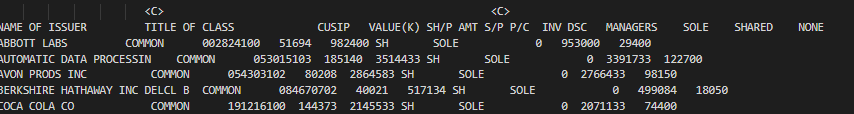
\includegraphics[width=0.8\textwidth]{13F_EX6.png}
    \caption[13F voorbeeld 7]{\label{fig:voorbeeld voor 2013 - inleiding}Een 13F-melding zonder gestructureerde data maar werkend met tabs, geen tabel structuur}
\end{figure}
Een voorbeeld van na 2013.

\begin{figure}[hbt!]
    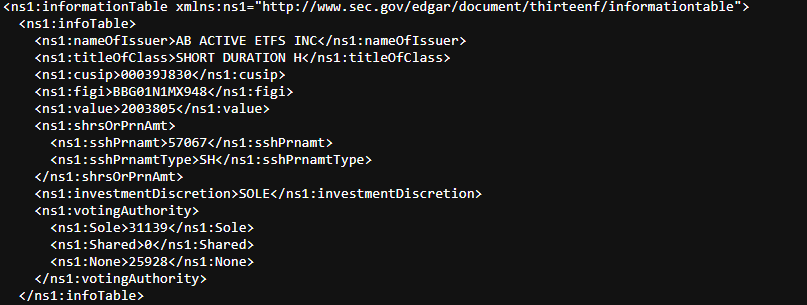
\includegraphics[width=0.8\textwidth]{13F_24_EX1.png}
    \caption[13F voorbeeld 7]{\label{fig:voorbeeld na 2013 - inleiding}Een recente (2024) 13F-melding gestructureerd in XML}
\end{figure}
\section{\IfLanguageName{dutch}{Onderzoeksvraag}{Research question}}%
\label{sec:onderzoeksvraag}

Hoe kunnen AI-technologieën zoals Text mining, Natural Language Processing (NLP) en Machine Learning (ML) effectief worden toegepast om 13F-meldingen van de SEC van voor 2013 te standaardiseren en te integreren in een gestructureerde databank, zodat de historische gegevens efficiënter kunnen worden geanalyseerd en vergeleken en is dit überhaupt mogelijk?

\section{Deelsonderzoekvragen}
\begin{enumerate}
    \item Welke specificaties en uitdagingen zijn verbonden aan 13F-meldingen van de SEC voor 2013?
    \item Hoe kunnen NLP-technologieën worden ingezet om de tekstuele gegevens in 13F-meldingen te extraheren en te standaardiseren?
    \item Wat zijn de praktische implicaties en voordelen van het standaardiseren en integreren van 13F-meldingen met behulp van AI-technologieën?
    
\end{enumerate}
\section{\IfLanguageName{dutch}{Onderzoeksdoelstelling}{Research objective}}%
\label{sec:onderzoeksdoelstelling}

Het hoofddoel van dit onderzoek is het ontwikkelen van een geautomatiseerde methode die gebruikmaakt van AI-technologieën, zoals NLP en ML, om de data uit de 13F-meldingen van voor 2013 te extraheren, standaardiseren en te integreren in een relationele databank. Dit moet leiden tot een efficiëntere en meer accurate extractie van gegevens uit deze documenten, waardoor de toegankelijkheid en bruikbaarheid van de data voor financieel onderzoek en investeringsanalyse aanzienlijk worden verbeterd. 
Het onderzoek stoelt op een POC te implementeren. Dit wil zeggen dat indien het omzettingsproces slaagt dit een aanleiding kan zijn om een volwaardige software tool te ontwerpen (door derden).


\section{\IfLanguageName{dutch}{Opzet van deze bachelorproef}{Structure of this bachelor thesis}}%
\label{sec:opzet-bachelorproef}

% Het is gebruikelijk aan het einde van de inleiding een overzicht te
% geven van de opbouw van de rest van de tekst. Deze sectie bevat al een aanzet
% die je kan aanvullen/aanpassen in functie van je eigen tekst.

Het verdere verloop van deze bachelorproef is opgebouwd als volgt:

In Hoofdstuk~\ref{ch:stand-van-zaken} wordt een overzicht gegeven van de stand van zaken binnen het onderzoeksdomein, op basis van een literatuurstudie.

In Hoofdstuk~\ref{ch:methodologie} wordt de methodologie toegelicht en worden de gebruikte onderzoekstechnieken besproken om een antwoord te kunnen formuleren op de onderzoeksvragen.
In Hoofdstuk~\ref{ch:benodigdheden}  worden de vereisten voor het ontwikkelen van de proof of concept besproken, inclusief een prioritering op basis van hun belang.
In Hoofdstuk~\ref{ch:proof of concept} wordt de proof of concept besproken. De inhoud omvat de ingewikkelde technische specificaties, structuur en tools, samen met de functionele elementen zoals de modellen en de databank.
In Hoofdstuk~\ref{ch:conclusie}, tenslotte, wordt de conclusie gegeven en een antwoord geformuleerd op de onderzoeksvragen. Daarbij wordt ook een aanzet gegeven voor toekomstig onderzoek binnen dit domein.